\documentclass{article}
\usepackage[utf8]{vietnam}
\usepackage{amsmath}
\usepackage{graphicx}
\graphicspath{ {./image/} }\usepackage{hyperref}
\title{TRUYEN SO LIEU VA MANG}

\begin{document}

Từ mã của các nodes: 
\begin{itemize}
\item 27: 000
\item 30: 00100
\item 20: 00101
\item 21: 0011
\item 25: 01
\item 23: 100
\item 22: 1010
\item 29: 10110
\item 28: 10111
\item 26: 110
\item 24: 111
\end{itemize}
Entropy:
\[
\sum_{i=0}^{k} \frac{\log{\left(\frac{1}{{p}_{i}} \right)} {p}_{i}}{\log{\left(2 \right)}} = 3.143
\]
Chiều dài TB từ mã:
\[
N = \sum_{i=0}^{k} {N}_{i} {p}_{i} = 3.179
\]
Hiệu suất Huffman:
\[
\frac{H}{N} = 0.989
\]
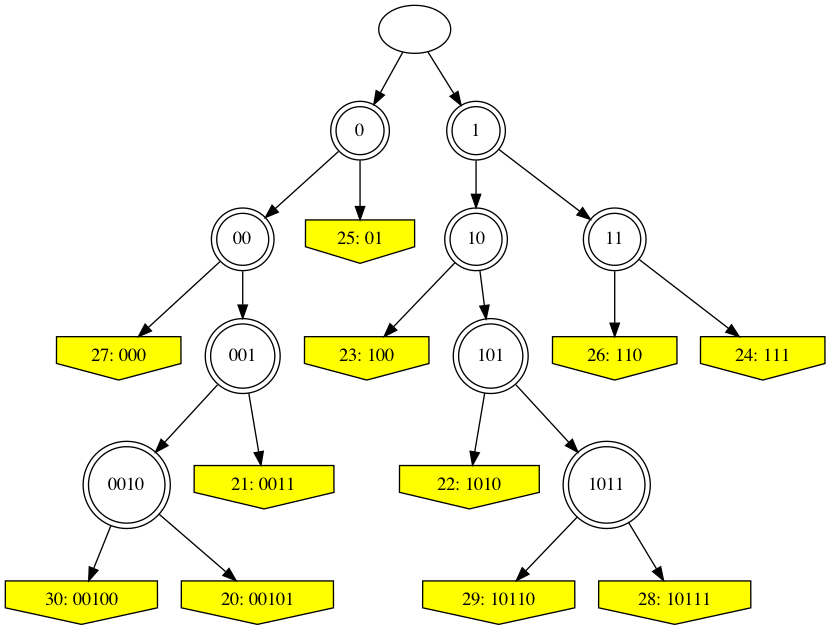
\includegraphics[width=\textwidth]{graph.png}
\begin{center}
\textit{Hình 1. Cây Huffman}
\end{center}
\end{document}
